%-----------------------------------------------
% Dateiname: CurrentSituation.tex
% Autor    : Stefano Kowalke <blueduck@gmx.net>
% Lizenz   : BSD
%-----------------------------------------------
\chapter{Aktuelle Situation}
\label{sec:currentSituation}
\section{Die native Datenbank API}
n Kapitel~\ref{basics:typo3:subsubsec:coreAndApi} wurde bereits darauf hingewiesen, dass die einheitliche Datenbank API von der Klasse \phpinline{\TYPO3\CMS\Core\Database\DatabaseConnection} bereitgestellt wird. Über die globale Variable \phpinline{$GLOBALS['TYPO3_DB']} kann darauf zugegriffen werden.

\begin{listing}[H]
	\begin{phpcode}
$GLOBALS['TYPO3_DB']->exec_UPDATEquery(
  $this->user_table,
  $this->userid_column . '=' .
    $this->db->fullQuoteStr(
      $tempuser[$this->userid_column],
      $this->user_table
    ),
  array($this->lastLogin_column => $GLOBALS['EXEC_TIME'])
);

	\end{phpcode}
	\caption{Aktualisierung des Zeitpunkts des letzten Logins}
	\label{lst:databaseOldExample}
\end{listing}

Durch die Nutzung der Datenbank API wird zum einen die Integrität der Daten sichergestellt und es werden die \gls{php}-Datenbankfunktionen abstrahiert. Somit kann die Implementation der API-Methoden angepasst werden, ohne die API selbst zu verändern. Auf diese Weise wurde die Umstellung von MySQL auf die MySQLi durchgeführt.\footnote{\url{http://bit.ly/typo3cms-switch-from-mysql-to-mysqli}}

Die Datenbank API bietet eine Vielzahl an Methoden, die sich in die folgenden fünf Gruppen einteilen lassen:

\begin{enumerate}
	\item Methoden die SQL-Abfragen generieren
	\item Methoden die SQL-Abfragen gegen die Datenbank ausführen
	\item Methoden die auf der Ergebnismenge agieren
	\item Administrative Methoden
	\item Hilfsmethoden
\end{enumerate}

\newpage

\subsection{Generierende Methoden}

Die erste Gruppe besteht aus Methoden, die anhand der übergebenen Parameter einen SQL-Abfrage generieren. Damit werden die typischen CRUD-Operationen~\ref{ft:crud} abgebildet.

\begin{figure}[H]
	\centering
	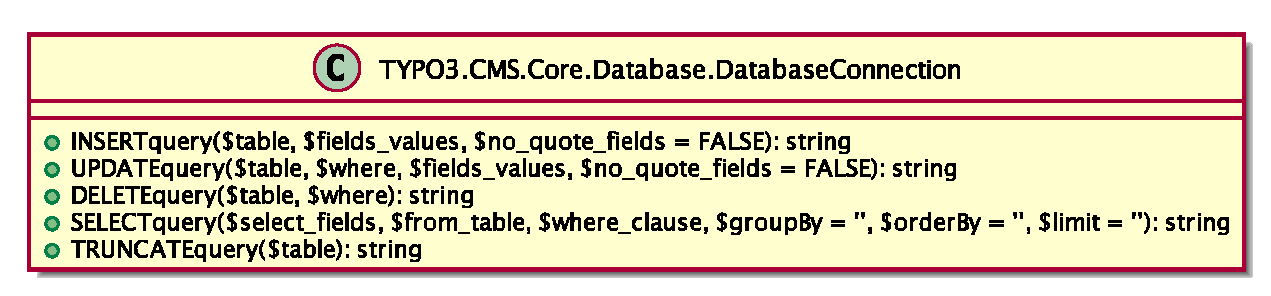
\includegraphics[scale=0.65]{gfx/uml/DatabaseConnectionCreationMethods.eps}
	\caption{Methoden zum Erzeugen von SQL-Abfragen}
	\label{fig:databaseConnectionWithSQLGenerationMethods}
\end{figure}

Folgendes Codebeispiel aus \phpinline{\TYPO3\CMS\Core\Authentication\AbstractUserAuthentication} zeigt die Funktionsweise von \phpinline{SELECTquery()}. Der Kommentar zeigt die generierte SQL-Abfrage.

\begin{listing}[H]
	\begin{phpcode}
// DELETE FROM sys_file_reference WHERE tablenames='pages';
$deleteQuery = $GLOBALS['TYPO3_DB']->DELETEquery(
    'sys_file_reference',
    'tablenames=' . $GLOBALS['TYPO3_DB']->fullQuoteStr(
      'pages',
      'sys_file_reference'
    )
);
	\end{phpcode}
	\caption{Löschen eines Datensatzes aus einer Tabelle}
	\label{lst:databaseOldDeleteExample}
\end{listing}

\subsection{Ausführende Methoden}
Eine Ebene höher setzt die nächste Gruppe an, die die eben gezeigten Methoden nutzt, den generierten SQL-Abfrage ausführt und eine Ergebnismenge vom Typ \phpinline{mysqli_result} zurückliefert.

\begin{figure}[H]
\centering
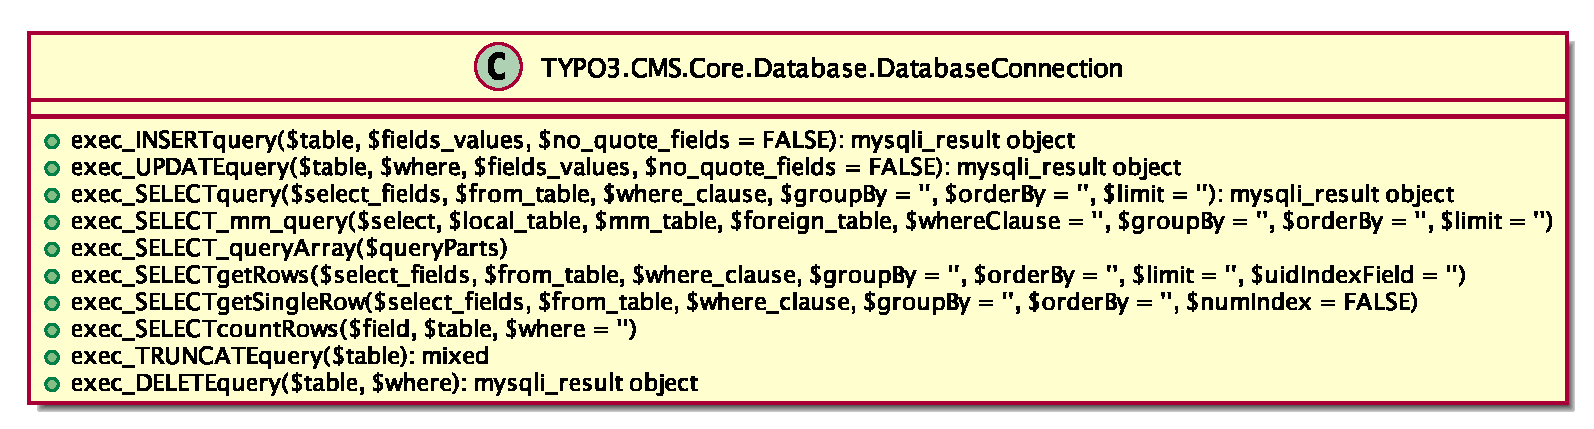
\includegraphics[scale=0.5]{gfx/uml/DatabaseConnectionExecuteMethods.eps}
\caption{Methoden zum Ausführen von SQL-Abfragen}
\label{fig:databaseConnectionWithSQLExecutionMethods}
\end{figure}

\newpage
\subsection{Methoden zur Manipulation der Ergebnismenge}
In der dritten Gruppe befinden sich die Methoden, die im weitesten Sinn zur Verarbeitung der Ergebnismenge genutzt werden. Darunter fallen

\begin{itemize}
	\item jene, die die Daten aus der Ergebnismenge extrahieren,
	\item die für die Fehlerbehandlung genutzt werden können,
	\item sowie Methoden, die Informationen über die Ergebnismenge bereitstellen
\end{itemize}

\begin{figure}[H]
\centering
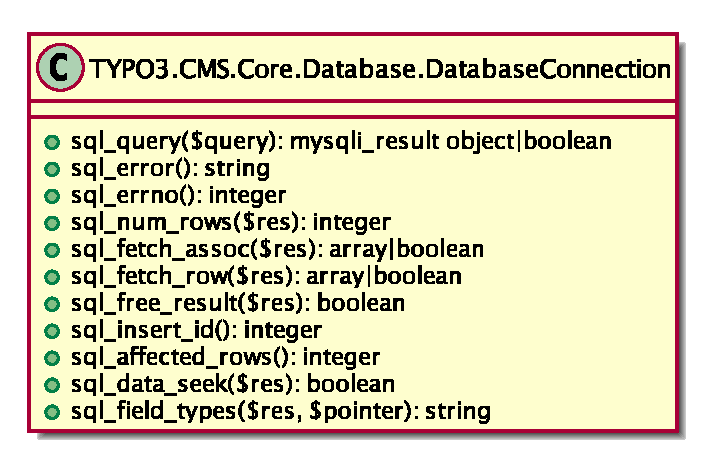
\includegraphics[scale=0.65]{gfx/uml/DatabaseConnectionFetchMethods.eps}
\caption{Methoden zur Verarbeitung der Ergebnismenge}
\label{fig:databaseConnectionWithResultsetsMethods}
\end{figure}


\subsection{Administrative Methoden}
Die nächste Gruppe besteht aus einer Reihe von Methoden, die verschiedene Metadaten über die Datenbank zur Verfügung stellen. Der Name impliziert, dass sie für Administrative Tätigkeiten genutzt werden, was jedoch irreführend ist. Sie werden hauptsächlich während der Installation vom \textit{Installation Tool} verwendet, um Informationen über die zugrundeliegende Datenbank zu erhalten

\begin{figure}[H]
\centering
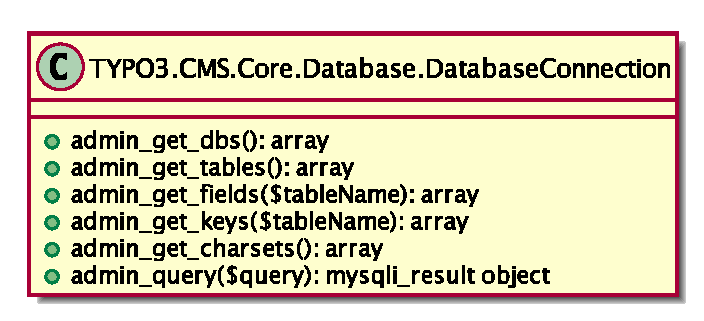
\includegraphics[scale=0.7]{gfx/uml/DatabaseConnectionAdminMethods.eps}
\caption{Administrativen Methoden}
\label{fig:databaseConnectionWithSQLAdminMethods}
\end{figure}

\newpage
\subsection{Hilfsmethoden}
Die letzte Gruppe besteht  aus Hilfsmethoden, die genutzt werden um

\begin{itemize}
	\item einen SQL-Abfrage an die Datenbank zu senden
	\item Benutzereingaben zu maskieren
	\item Listen von Integern zu normalisieren
	\item eine \phpinline{WHERE}-Bedingung aus Komma-separierten Datensätzen zu erzeugen
\end{itemize}

\begin{figure}[H]
\centering
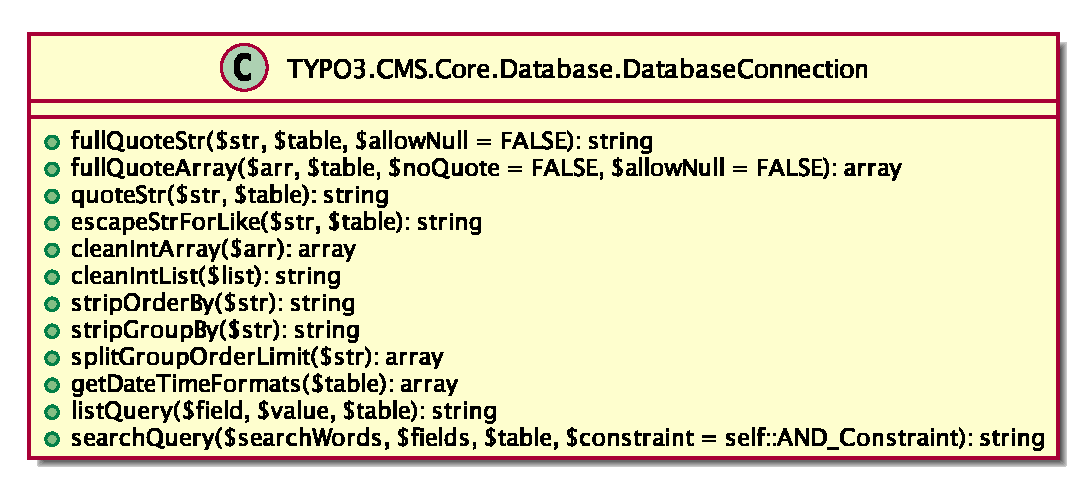
\includegraphics[scale=0.65]{gfx/uml/DatabaseConnectionHelperMethods.eps}
\caption{Hilfsmethoden}
\label{fig:databaseConnectionWithHelperMethods}
\end{figure}

\section{Prepared Statements}
\label{currentsituationsubsec:preparedStatements}
Seit TYPO3 CMS 4.5 können Prepared Statements für \mysqlinline{SELECT} Abfragen verwendet werden. TYPO3 CMS unterstützt sowohl \textit{Posistional Parameters} wie auch \textit{Named Parameters}.

\begin{listing}
\begin{phpcode}
$statement = $GLOBALS['TYPO3_DB']->prepare_SELECTquery(
  '*', 'bugs', 'reported_by = ? AND bug_status = ?'
);
$statement->execute(array('goofy', 'FIXED'));

$statement = $GLOBALS['TYPO3_DB']->prepare_SELECTquery(
  '*', 'bugs', 'reported_by = :nickname AND bug_status = :status'
);
$statement->execute(array(':nickname' => 'goofy', ':status' => 'FIXED'));
\end{phpcode}
\caption{Positional und Named Prepared Statements der TYPO3 CMS Datenbank API}
\label{lst:databaseOldPreparedStatement}
\end{listing}

\phpinline{\TYPO3\CMS\Core\Database\DatabaseConnection::prepare_SELECTquery} liefert ein Objekt der Klasse \phpinline{\TYPO3\CMS\Core\Database\PreparedStatement} zurück, welches sich an der API von \gls{pdo} orientiert.

\begin{figure}[H]
    \centering
    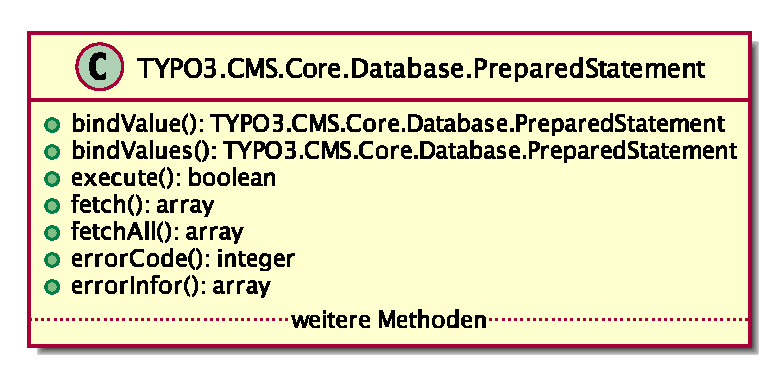
\includegraphics[scale=0.75]{gfx/uml/PreparedStatement.eps}
    \caption{Die Klasse PreparedStatement mit ausgewählten Methoden}
    \label{fig:selectedMethodsOfPreparedStatements}
\end{figure}

\section{Datenbankschema}
\label{currentSituation:subsec:databaseSchema}
Nach der Installation von TYPO3 CMS beinhaltet die Datenbank rund 60 einzelne Tabellen. Die Anzahl hängt von der Installation der optionalen Systemextensions ab.

Wichtige Tabellen sind:
\begin{itemize}
	\item pages – Enthält die Seiten
	\item tt\_content – Enthält die Inhaltselemente, die auf den Seiten dargestellt werden
	\item be\_groups / fe\_groups – Enthält die Backend- beziehungsweise die Nutzergruppen
	\item be\_users / fe\_users – enthält die Backend- beziehungsweise die Frontendbenutzer
\end{itemize}

Dazu kommen Tabellen
\begin{itemize}
	\item die gecachte Daten und Sessions beinhalten,
	\item die der Indexierung des Inhalts dienen
	\item sowie zum Protokollieren von Systemereignissen
\end{itemize}

Die Inhalte werden in TYPO3 CMS in einer Dateisystem ähnlichen Baumstruktur verwaltet. Eine Webseite wird darin durch einen Datensatz vom Typ \textit{Seite} repräsentiert. Dieser Datensatz hat eine ID, die im gleichnamigen Feld in der Tabelle \texttt{pages} gespeichert wird. Diese ist der \textit{Unique Identifier} des Datensatzes.

Die Inhalte einer Webseite wie Texte, Bilder oder Formulare werden innerhalb einer Seite abgelegt. TYPO3 CMS bietet hierzu eine breite Palette von verschiedenen Elementen an. Zudem können Plugins und wiederum Seiten innerhalb eines Seitendatensatzes abgelegt werden. Diese Liste kann unbegrenzt fortgeführt werden, da jede Extension neue Elemente einführen kann, die in einer Seite ablegbar sind. Es ist lediglich wichtig zu wissen, dass Datensätze innerhalb von Seiten abgelegt werden können. Die Inhaltselemente werden hauptsächlich in der Tabelle \texttt{tt\_content} gespeichert beziehungsweise in den Tabellen, die die Extension vorsieht.

\begin{figure}[H]
	\centering
	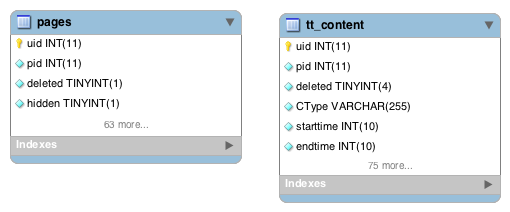
\includegraphics[scale=0.6]{diagrams/DatabasePagesTTContent.png}
	\caption{Die Tabellen pages und tt\_content}
	\label{fig:pagesAndTTContent}
\end{figure}

Die Verknüpfung von Inhaltselement zu übergeordneter Seite erfolgt in der Datenbank über die Spalte \phpinline{pid} (PageID), in der die ID der übergeordneten Seite als Fremdschlüssel gespeichert wird. Listing~\ref{lst:getSubpages} zeigt die SQL-Abfrage, die alle Unterseiten einer Seite zurückgibt. Dabei hat die Seite, dessen Unterseiten abgefragt werden, die \texttt{uid} 4, die in die Abfrage eingesetzt wird. Die Abfrage lautet: Wähle alle Datensätze aus der Tabelle \texttt{pages}, die in der Spalte \texttt{pid} eine 4 stehen haben.

\begin{listing}
	\begin{phpcode}
SELECT * FROM pages WHERE pid=4 ORDER BY sorting
	\end{phpcode}
	\caption{Abrufen von Unterseiten einer Seite}
	\label{lst:getSubpages}
\end{listing}

Analog zum vorigen Listing, zeigt das Folgende die SQL-Abfrage, die alle Inhaltselemente von der Datenbank abfragt.

\begin{listing}
	\begin{phpcode}
SELECT * FROM tt_content WHERE pid=4 ORDER BY sorting
	\end{phpcode}
	\caption{Abrufen von Inhaltselementen einer Seite}
	\label{lst:getContentElements}
\end{listing}

Die beiden Abfragen geben alle Datensätze zurück, was in der Realität jedoch meistens nicht gewünscht ist. Zum Beispiel sollen keine gelöschten Datensätze angezeigt oder nicht alle Inhaltselemente ausgegeben werden. Datensätze werden in der Datenbank nicht gelöscht, sondern in der Spalte \textit{deleted} durch das setzen des Wertes auf 1 als gelöscht markiert. Inhaltselemente werden über die Spalte \texttt{CType} nach ihrem Typ gefiltert. Um das gewünschte Ergebnis zu erhalten müssen \mysqlinline{WHERE}-Klauseln formuliert werden, was die doch recht trivialen SQL-Abfragen schnell komplex werden lässt.

In TYPO3 CMS können die Benutzerrechte sehr granular eingestellt werden. Die Einstellungen können per Benutzer oder Benutzergruppe vorgenommen werden.
Dabei kann ein Benutzer Mitglied keiner, einer oder mehrerer Benutzergruppen sein. Zudem kann eine Benutzergruppe keinen, einen oder mehrere Benutzer enthalten. Dies stellt eine Many-to-Many-Relation dar.

In der Datenbank wird die Zugehörigkeit von Benutzer zu Gruppe von den Tabellen \texttt{fe\_users} und \texttt{fe\_groups} beziehungsweise \texttt{be\_users} und \texttt{be\_groups} abgebildet.

\begin{figure}[H]
	\centering
	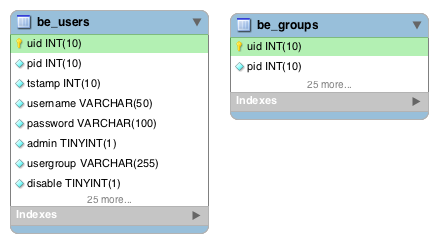
\includegraphics[scale=0.6]{diagrams/DatabaseBEUserGroup.png}
	\caption{Die Tabellen be\_users und be\_groups}
	\label{fig:beUsersAndBeGroups}
\end{figure}

In Abbildung~\ref{fig:beUsersAndBeGroups} fällt der Datentyp der Spalte \texttt{usergroup} auf, der die ID der Gruppe des Benutzers speichert. Er wurde als Typ \mysqlinline{VARCHAR} definiert, obwohl die Spalte \texttt{uid} den Typ \mysqlinline{INT} hat. Dies liegt darin, dass die Zuordnung der Benutzer zu Gruppe über eine kommaseparierte Liste erfolgt:

\begin{table}[H]
\begin{Verbatim}[samepage=true]
+----+-----+------------+----------+----------+-------+-----------+---------+
| id | pid |   tstamp   | username | password | admin | usergroup | deleted |
+----+-----+------------+----------+----------+-------+-----------+---------+
|  1 |  0  | 1191353353 | admin    |  secret  |   1   |           |    0    |
|  2 |  0  | 1281556682 | snape    |  secret  |   1   |    43     |    0    |
|  3 |  0  | 1191353353 | hagrid   |  secret  |   0   |  5,32,43  |    0    |
+----+-----+------------+----------+----------+-------+-----------+---------+
\end{Verbatim}
\caption{Auszug aus der be\_users Tabelle}
\label{tab:tableBeUser}
\end{table}

Kommaseparierte Listen gibt es an vielen Stellen in der Datenbank. Die API von TYPO3 CMS stellt Methoden bereit, die die Liste für die weitere Verarbeitung aufbereiten.

Dieses Konstrukt existiert wahrscheinlich seit Beginn des Systems und es ist zu vermuten, dass damit eine Many-to-Many-Tabelle vermieden werden sollte, was die Komplexität der SQL-Abfrage erhöht.

Um die kommaseparierten Listen aufzulösen, müsste eine weitere Tabelle eingeführt werden, deren zwei Spalten jeweils auf die \texttt{id} der beiden zu verknüpfenden Tabellen referenzieren.

\begin{figure}[H]
	\centering
	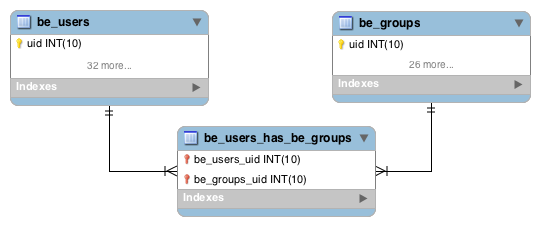
\includegraphics[scale=0.6]{diagrams/DatabaseBEUserGroupMM.png}
	\caption{Normalisierung über Many-to-Many Tabelle}
	\label{fig:beUsersHasBeGroups}
\end{figure}

\begin{table}[H]
\begin{Verbatim}[samepage=true]
+--------------+---------------+
| be_users_uid | be_groups_uid |
+--------------+---------------+
|      2       |      34       |
|      3       |       5       |
|      3       |      32       |
|      3       |      43       |
+--------------+---------------+
\end{Verbatim}
\caption{Die MM-Tabelle für be\_users}
\label{tab:mmTableBeUser}
\end{table}

TYPO3 CMS nutzt weder Datenbankseitige \textit{Constraints} noch Fremdschlüssel Definitionen. Alle Referenzierungen werden von TYPO3 CMS selbst verwaltet.
